\documentclass[a4paper]{llncs}

\usepackage{xcolor}
\usepackage{amsmath} 
\usepackage{hyperref}
\usepackage{graphicx}
\usepackage{subcaption}
\usepackage{booktabs}
\usepackage{siunitx}
\usepackage{pgfplotstable}

\sisetup{
  round-mode          = places, 
  round-precision     = 5, 
}
   
\hypersetup{
    colorlinks=true,
    linkcolor=magenta,
    urlcolor=blue,
    breaklinks,
    citecolor=blue
}

\pgfplotstableset{
  multistyler/.style 2 args={
    @multistyler/.style={display columns/##1/.append style={#2}},
    @multistyler/.list={#1}
  }
}


\newcommand{\bracketR}[1]{\left(#1\right)}
\newcommand{\bracketS}[1]{\left(#1\right)}
\newcommand{\bracketC}[1]{\left(#1\right)}
\newcommand{\innerproduct}[1]{\left<#1\right>}
\newcommand\norm[1]{\left\lVert#1\right\rVert}


\newcommand{\guy}[1]{\marginpar{\textcolor{orange}{Guy: #1}}}
\newcommand{\ben}[1]{\marginpar{\textcolor{blue}{Ben: #1}}}

\begin{document}


\title{Verifying the Resilience of Neural Network Watermarking}

\author{
  Ben Goldberger\inst{1} \and
  Yossi Adi\inst{2} \and
  Joseph Keshet\inst{2} \and
  Guy Katz\inst{1} 
}

\institute{
  The Hebrew University of Jerusalem, Israel \\
  \{jjgold, guykatz\}@cs.huji.ac.il
  \and
Bar Ilan University, Israel \\
\{a, b\}@biu.ac.il
}

\maketitle

\section{Introduction}

% Each of these should be extended into 1-2 paragraphs

Deep Neural Networks (DNN) are a nowadays phenomena in research and in Industry; They're used for large verity of applications, and achieving state of the art result in many fields (Computer vision, speech recognition, AI, and many more). DNNs flexibility and diversity are pushing the limits on what is possible for a computer to solve efficiently. As a result from their empiric success DNNs are now changing the way software is being designed, and broaden the role of Machine Learning trained functions in applications.

Because of the success of DNNs and because designing and training a DNN require certain expertise, time and processing power, the demand for a specifically designed DNN is growing, And Machine Learning as a Service (MLaaS) is now a thing. There are many machine learning services appearing in many forms, from data visualization and cloud computing to frameworks and semi-trained DNNs. This create some issues regarding the rights and ownership of some part of a trained network or design. Because of the relatively simple components of a DNN (Matrices, vectors and simple functions) it's quite easy to copy or use without permission.

In order to deal with such issues we need a way to authenticate a DNN. This may sound simple but the authentication needs to be robust, such that it's hard to remove. Here comes the concept of Digital Watermarking, a way of signing some Digital property such that it's hard to remove the signature, and said signature is unique. There are some proposed method of watermarking a DNN, but it's unclear how effective they are, meaning how difficult it is to remove the watermark from the DNN and what is the effect of removing the watermark.

DNN verification is a new and promising field. We propose a novel
methodology to use verification to measure and verify the robustness
of watermarking techniques.
Main uses of our approach: verify watermarked networks, assess
efficiency of watermarking schemes.

The rest of this paper is organized as follows. In
Section~\ref{sec:background} we provide the necessary background on
DNNs, watermarking, and DNN verification. Next, in
Section~\ref{sec:verifyWatermarks} we introduce our technique for
casting the watermark resilience problem into a verification
problem. Section~\ref{sec:evaluation} describes our implementation and evaluation of the approach on several watermarked DNNs for image
recognition. We discuss related work in Section~\ref{sec:relatedWork},
and conclude in Section~\ref{sec:conclusion}.

\section{Background}
\label{sec:background}

\cite{KaBaDiJuKo17Reluplex,KaHuIbJuLaLiShThWuZeDiKoBa19Marabou}

\section{Finding the minimal change that will get rid of the network's WaterMark}
\label{sec:verifyWatermarks}

Given a watermarked trained neural network as described
here \cite{AdBaPiKeWatermarking}.
\guy{make this a proper citation}
\ben{ok}
We
tested what is the minimal change to the network last layer in order
to "remove" some watermarks from the network.


\subsection{Defining the problem for one input}
\label{sec:defineProblem1}

Given a watermarked network $N$ with a set of $K$ watermarks (A set of
inputs to the network) $\bracketsC{x_1,\cdots,x_K}$ we'll mark the network last layer matrix $L$ such that $L$ is a $m\times n$ matrix were $n$
is the layer's number of neurons and $m$ is the network output size.
The change to the last layer will be a matrix with the same dimension
as $L$ we'll mark as $\varepsilon$, such that $\varepsilon_{i,j}$ is the change to the last layer matrix entry $L_{i,j}$. We can describe the network output as  
For a certain input $x$ we're only interested in the input to the last layer we'll mark the input to the last layer $v$. $v$ is a $n\times 1$
vector.  So the original network output $y = Lv$ and the changed
network output is $y' = (L+\varepsilon)v$.
\\\\
For a single input $x$ we denote the original network prediction:
$$
   	d_x := argmax_{i\in \bracketsS{m}}\bracketsC{y_i}
$$
And the changed network prediction:
$$
   	d'_x := argmax_{i\in \bracketsS{m}}\bracketsC{y'_i}
$$
\\
We're interested to find the minimal change to the last layer $\varepsilon$  so that the prediction will change i.e. $d_x\neq d'_x$
\\\\
Well measure the overall change to the layer in two ways
\begin{equation}
\label{eq:normInf}
	\begin{split}
   		\norm{\varepsilon}_{\infty}=max_{i,j}\bracketsC{\abs{\varepsilon_{i,j}}}.
	\end{split}
\end{equation}
And
\begin{equation}
\label{eq:normOne}
	\begin{split}
   		\norm{\varepsilon}_1=\sum_{i,j}\abs{\varepsilon_{i,j}}.
	\end{split}
\end{equation}
\\
For the $\ell_\infty-norm$ \ref{eq:normInf} and a chosen $d'_x$ that is different from $d_x$ the minimization problem looks like that:
\begin{equation}
\label{eq:LP}
\begin{split}
    Minimize:\quad & M \\
    Subject\ to:\quad & \forall i,j\quad -M \leq\varepsilon_{i,j}\leq M \\
    & y'=(L+\varepsilon)v \\
    & y'_{d_x} \leq y'_{d'_x} \\
	\intertext{Variables are the entries in $\varepsilon,y'$ and $M$}
\end{split}
\end{equation}
\\\\
Similarly for the $\ell_1-norm$ \ref{eq:normOne} the minimization problem looks like that:
\begin{equation}
\label{eq:NotLP}
\begin{split}
    Minimize:\quad & M \\
    Subject\ to:\quad & \forall i,j\quad -M \leq\sum_{i,j}\abs{\varepsilon_{i,j}}\leq M \\
    & y'=(L+\varepsilon)v \\
    & y'_{d_x} \leq y'_{d'_x} \\
	\intertext{Variables are the entries in $\varepsilon,y'$ and $M$}
\end{split}
\end{equation}
\subsection{Defining the problem for many inputs}
\label{sec:defineProblem2}

Our definition to a single input minimal change $\varepsilon$ to the network last layer $L$ can be extended to more then one input very easily by adding more constraint to the problem.
\\
Given inputs $\bracketsC{x_1,\cdots,x_k}$ and their respective values:
\begin{align*}
\bracketsC{v_1,\cdots,v_k}\quad: & \text{Inputs to the last layer} \\
\bracketsC{y_1,\cdots,y_k}\quad: & \text{Output vectors} \\
\bracketsC{d_1,\cdots,d_k}\quad: & \text{Decisions} \\
\intertext{Such that}
\forall 1\leq j\leq k\quad & d_j \neq argmax_{i\in\bracketsS{m}}\bracketsC{\bracketsR{\bracketsR{L+\varepsilon}v_j}_i}
\end{align*}
\\
Assuming we choose our new desired decisions
$\bracketsC{d'_1,\cdots,d'_k}$ our minimization problem for the $\infty-norm$ looks like this:
\begin{equation}
\label{eq:LPmany}
\begin{split}
    Minimize:\quad & M \\
    Subject\ to:\quad & \forall i,j\quad -M \leq\varepsilon_{i,j}\leq M\\
    & \forall j\quad y'_j=(L+\varepsilon)v_j \\
    & \forall j\quad \bracketsR{y'_j}_{d_j} \leq \bracketsR{y'_j}_{d'_j}\\
	\intertext{Variables are the entries in $\varepsilon,y'_1,\cdots,y'_k$ and $M$}
\end{split}
\end{equation}
Similarly for the $\ell_1-norm$ \ref{eq:normOne} the minimization problem looks like that:
\begin{equation}
\label{eq:NotLPmany}
\begin{split}
    Minimize:\quad & M \\
    Subject\ to:\quad & \forall i,j\quad -M \leq\sum_{i,j}\abs{\varepsilon_{i,j}}\leq M\\
    & \forall j\quad y'_j=(L+\varepsilon)v_j \\
    & \forall j\quad \bracketsR{y'_j}_{d_j} \leq \bracketsR{y'_j}_{d'_j}\\
	\intertext{Variables are the entries in $\varepsilon,y'_1,\cdots,y'_k$ and $M$}
\end{split}
\end{equation}

\guy{Overall, this looks good. Some stuff will need to be moved to other
sections according to the paper layout.}

\section{Evaluation}
\label{sec:evaluation}
For the $\ell_\infty-norm$ \ref{eq:normInf} when choosing a prediction different from the original the problem can be expressed as a linear programming query. This is possible since $y'=(L+\varepsilon)v$ is a linear set of constraint, and each entry of $\varepsilon$ can be bounded independently.
\\


We tested this approach on a Neural network trained on the MNIST data set, the network was watermarked with $100$ images of Gaussian noise. The original network had $96.8\text{\%}$ accuracy on the MNIST test set and $100\text{\%}$ accuracy on the watermark images.

\begin{figure}[h!]
  \centering
  \begin{subfigure}{0.4\linewidth}
    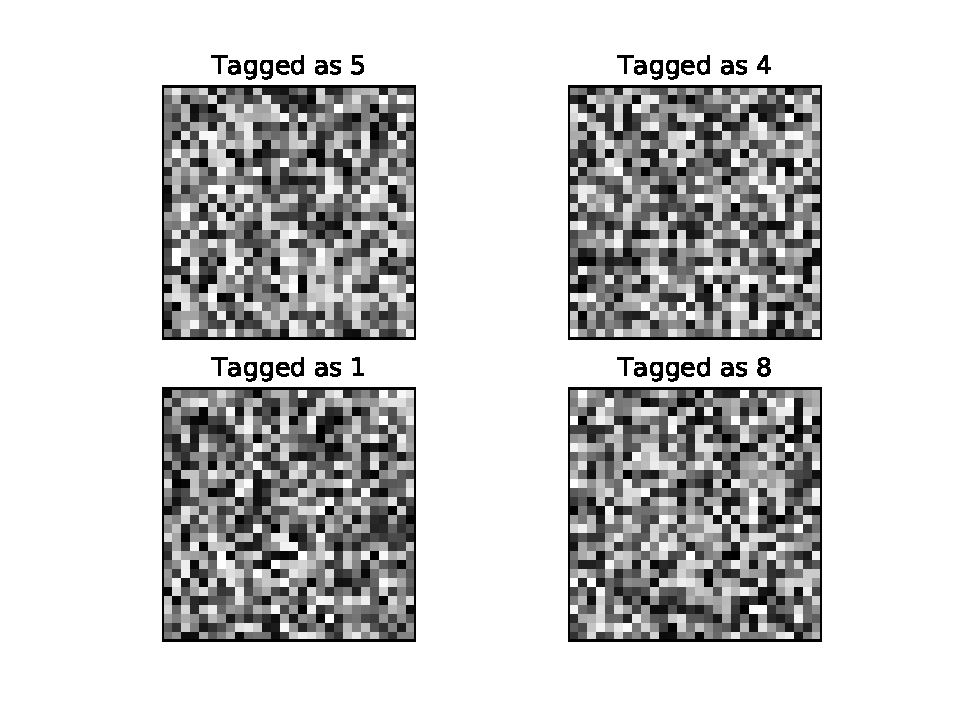
\includegraphics[width=\linewidth]{../data/wm.pdf}
     \caption{Water marks images.}
  \end{subfigure}
  \begin{subfigure}{0.4\linewidth}
    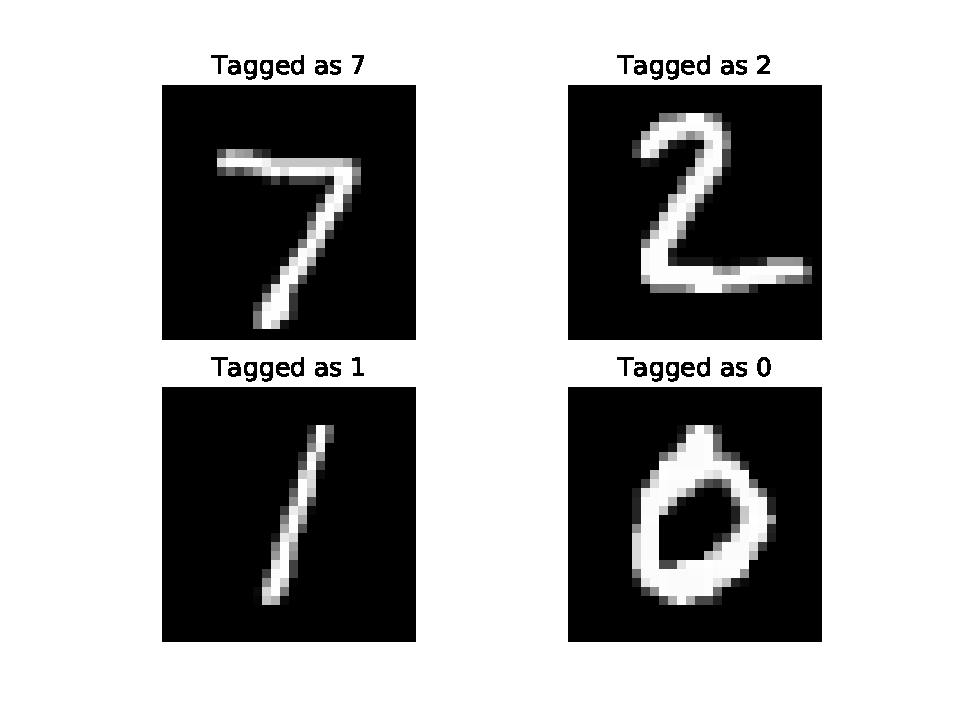
\includegraphics[width=\linewidth]{../data/mnist.pdf}
    \caption{MNIST images.}
  \end{subfigure}
  \label{fig:imageExamples}
\end{figure}

\subsection{Removing a single watermark}
The first test we did was to find the minimal change according to $\norm{\cdot}_{\infty}$ norm and $\norm{\cdot}_1$ norm for every water mark image as describe~\ref{sec:defineProblem}. We choose to change the original tagging of the image to the second highest score that image got. For example an image $w$ with an output $y$ 
$$j=\underset{i\in\bracketsC{0,\cdots,9}}{argmax}\bracketsC{y_i}$$ 
$j$ is the original tagging of $w$. 
$$j'=\underset{i\in\bracketsC{0,\cdots,9}\setminus \bracketsC{j}}{argmax}\bracketsC{y_i}$$ 
$j'$ is the new tagging of $w$. \\\\
meaning that after we change the last layer of the network the new output $y'$ largest coordinate is $j'$.   
Each watermark image have different minimal $\varepsilon$. This can give us some measure of how difficult it is to remove a single watermark image.

\begin{figure}[h!]
  \centering
  \begin{subfigure}{0.4\linewidth}
    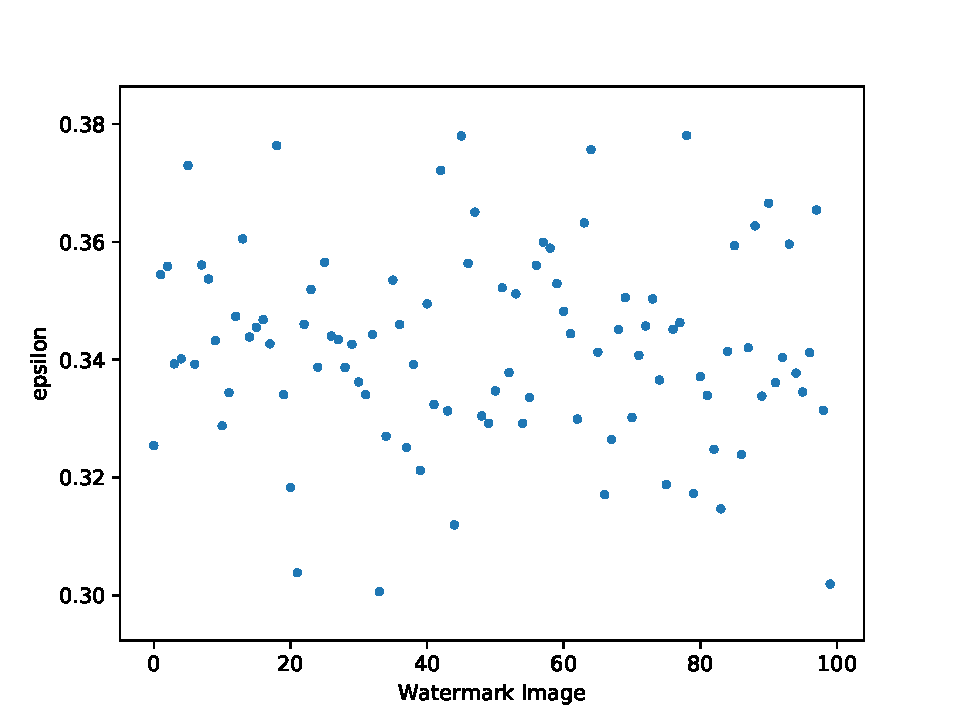
\includegraphics[width=\linewidth]{../data/results/problem3/mnist_w_wm.pdf}
     \caption{The Minimal $\norm{\cdot}_{\infty}$ for every watermark image}
  \end{subfigure}
  \begin{subfigure}{0.4\linewidth}
    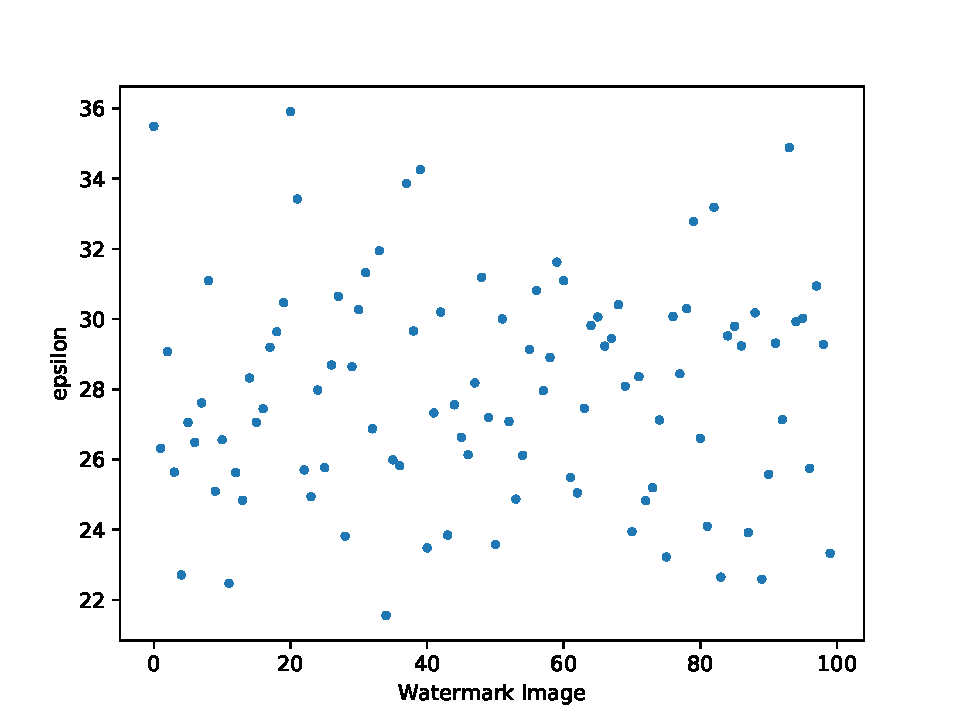
\includegraphics[width=\linewidth]{../data/results/problem2/mnist_w_wm.pdf}
    \caption{The Minimal $\norm{\cdot}_1$ for every watermark image}
  \end{subfigure}
  \label{fig:minimalEpsilonSingle}
  \caption{Notice the scale of the graphs, the $\norm{\cdot}_\infty$ values are much smaller then the $\norm{\cdot}_1$ values. As expected}
\end{figure}

After removing a single watermark with minimal change to the last layer we're interested in the effect this had on our original network accuracy. To test the accuracy after we found the changes all we had to is apply the changes to the original network and run an evaluation on the original network dataset.
As seen in this table \ref{table:singleWatermark} the $\norm{\cdot}_1$ gives better accuracy result on average by can have a bad accuracy result, and the $\norm{\cdot}_\infty$ after removing a single watermark have a consistent result (there minimal accuracy and the maximal accuracy are quite close)

\begin{table}[h!]
  \begin{center}
    \caption{Epsilons and Accuracy}
    \pgfplotstabletypeset[
    	  col sep=comma,
      multistyler={0,...,6}{column type={c|}},
      columns/Norm/.style={string type},
    	]{../data/results/mnist_w_wm_1_wm.csv}
  \end{center}
  \label{table:singleWatermark}
\end{table}

\begin{figure}[h!]
  \centering
  \begin{subfigure}{0.4\linewidth}
    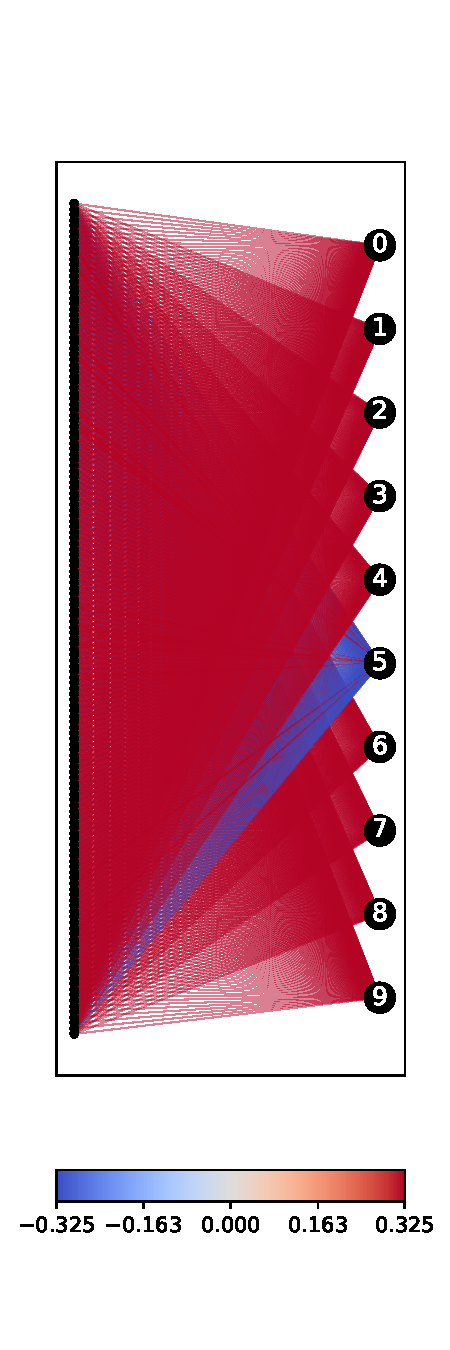
\includegraphics[width=\linewidth]{../data/results/problem3/last_layer_1_wm_example.pdf}
     \caption{The Minimal $\norm{\cdot}_{\infty}$ for every watermark image}
  \end{subfigure}
  \begin{subfigure}{0.4\linewidth}
    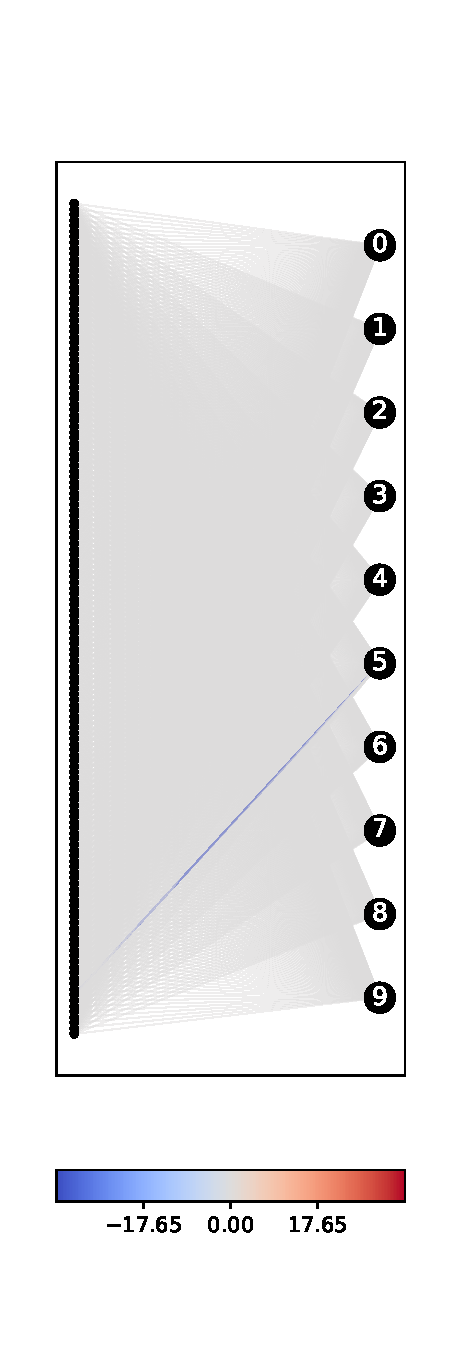
\includegraphics[width=\linewidth]{../data/results/problem2/last_layer_1_wm_example.pdf}
    \caption{The Minimal $\norm{\cdot}_1$ for every watermark image}
  \end{subfigure}
  \label{fig:lastLayerExample1}
\end{figure}


\subsection{Removing Multiple watermark}

Removing a single 


\section{Related Work}
\label{sec:relatedWork}

\section{Conclusion and Future Work}
\label{sec:conclusion}


\bibliographystyle{abbrv}
\bibliography{watermarks}

\end{document}

%%% Local Variables:
%%% mode: latex
%%% TeX-master: t
%%% End:
